%% Document initiation %%
\documentclass[11pt]{article}
\usepackage[utf8]{inputenc}
\usepackage[a4paper, total={6.3in, 9.7in}]{geometry}
\setlength{\parskip}{1em}


%% Package Declarations %%
\usepackage{amssymb,amsmath, algorithm, algorithmic}
\usepackage{xcolor, times,psfrag,epsf,epsfig,graphics, tabularx, array}
\usepackage{tikz}
\usepackage{multicol, wrapfig, ctable}
\usepackage{fancyhdr, hanging, setspace}


%% Comman Declarations %%
\newcommand\mybox[2][]{\tikz[overlay]\node[fill=blue!20,inner sep=2pt, anchor=text, rectangle, rounded corners=1mm,#1] {#2};\phantom{#2}}
\renewcommand{\arraystretch}{1.2}

\pagestyle{fancy}
\setstretch{2.2}
\begin{document}

%% Document Building %%
\graphicspath{{images/}}

%% Title %%
\title{Relativistic Runaway Electrons and Lightning Discharge: a Qualitative Overview}
\author{William Jardee}
\date{\today}
\maketitle


\begin{multicols*}{2}
    

    \noindent
{\bf \LARGE Introduction}

    One of the favorite facts many people trying to inspire young minds towards studying physics, is the concept that we have little idea of how lightning strikes actually happen (this was one of the initial curiosities that inspired me as a kid). While this is true, we do understand little about the fine details of the mechanics that drive lightning strikes, especially how they are initiated, within the last couple decades a new, promising theory has been developed to explain events like lightning initiation. Much of the effective literature on the topic has been developed by two separate groups: for theory A. V. Gurevich's group in Russia leads the charge, on science communication and computational/observational analysis J. R. Dwyer is the primary group leader. I set out to begin understanding the introductory premise of two primary questions that have yet to be comprehensively answered:
    \begin{enumerate}
            \item By what physical mechanisms is lightning initiated, and how do these mechanisms related to step leaders?
            \item What physics describes X-ray flashes and other powerful emission events seen from thunderclouds and how is this physics related to the mechanisms that initiate lightning strikes, both cloud to ground and compact intra-cloud discharges (CIDs)? 
    \end{enumerate}

    These ideas are all wrapped up in a "rapidly expanding field of energetic particle and radiation physics in terrestrial and planetary atmospheres, and their effects" which Dwyer coined "high-energy atmospheric particle physics." The fundamental idea was first proposed by C.T.R. Wilson in 1925 with his theory of Runaway Electrons, relativistic particles in a fluid that are able to accelerate into lower energy states. This idea sat mostly dormant until 1992-2001 when a mad dash for a kinetic theory of this phenomena took off with new computational possibilities of the modern computer. In the mid 2000s the focus of research shifted to trying to understand what type of catalysts were required in these events. Since then progress has slowed down as scientists work out kinks and improve Monte Carlo modeling to better fit our observed data. I will go over the necessity of RREs (relativistic runaway electrons) in thunderclouds, how they exponentially grow into an avalanche event with numerous feedback loops, and what type of conditions are required to allow the events to happen at all. Then, I will explore what type of photon emissions are thought to come from these RRE events and how they can be used to model step leaders. Finally I will give a quick overview of the current stance of the theory with respect to current computational models and observational data. 
    \newline
    

    \noindent
{\bf \LARGE Background Physics}

    Before we delve into Relativistic Runaway Electrons, we must first establish a base understanding of storm clouds. The simplest depiction of a storm cloud is a type of tripole, where the top, middle and bottom of cloud are charged. The typical charge distribution has about 40 coulombs of charge at the top, -40 coulombs in the middle, and 3 coulombs at the bottom (see figure 1 for a visual depiction). Notice how this will create two net electric fields within the cloud: one pointing down towards the center and another point up also towards the center. Along the outside surface of the cloud a thin layer of negative charge accumulates because of the conductivity of the nearby air, however this effect won't play a meaningful role in the runaway phenomena. While the charges and layout of the tripole can vary, the most typical cloud is what is drawn here and will be the basis for nearly all the theories developed. Storm clouds discharge through many different types of lightning strikes from cloud to ground, ground to cloud, intra-cloud (inside the counts mass), etc.$^{(5)}$ While all strikes appear and hold some significance to the story of lightning physics, the most common ones are cloud to ground and intra-cloud strikes. Because these are the most common strikes they will be focus of our talks.
    
    \begin{center}
        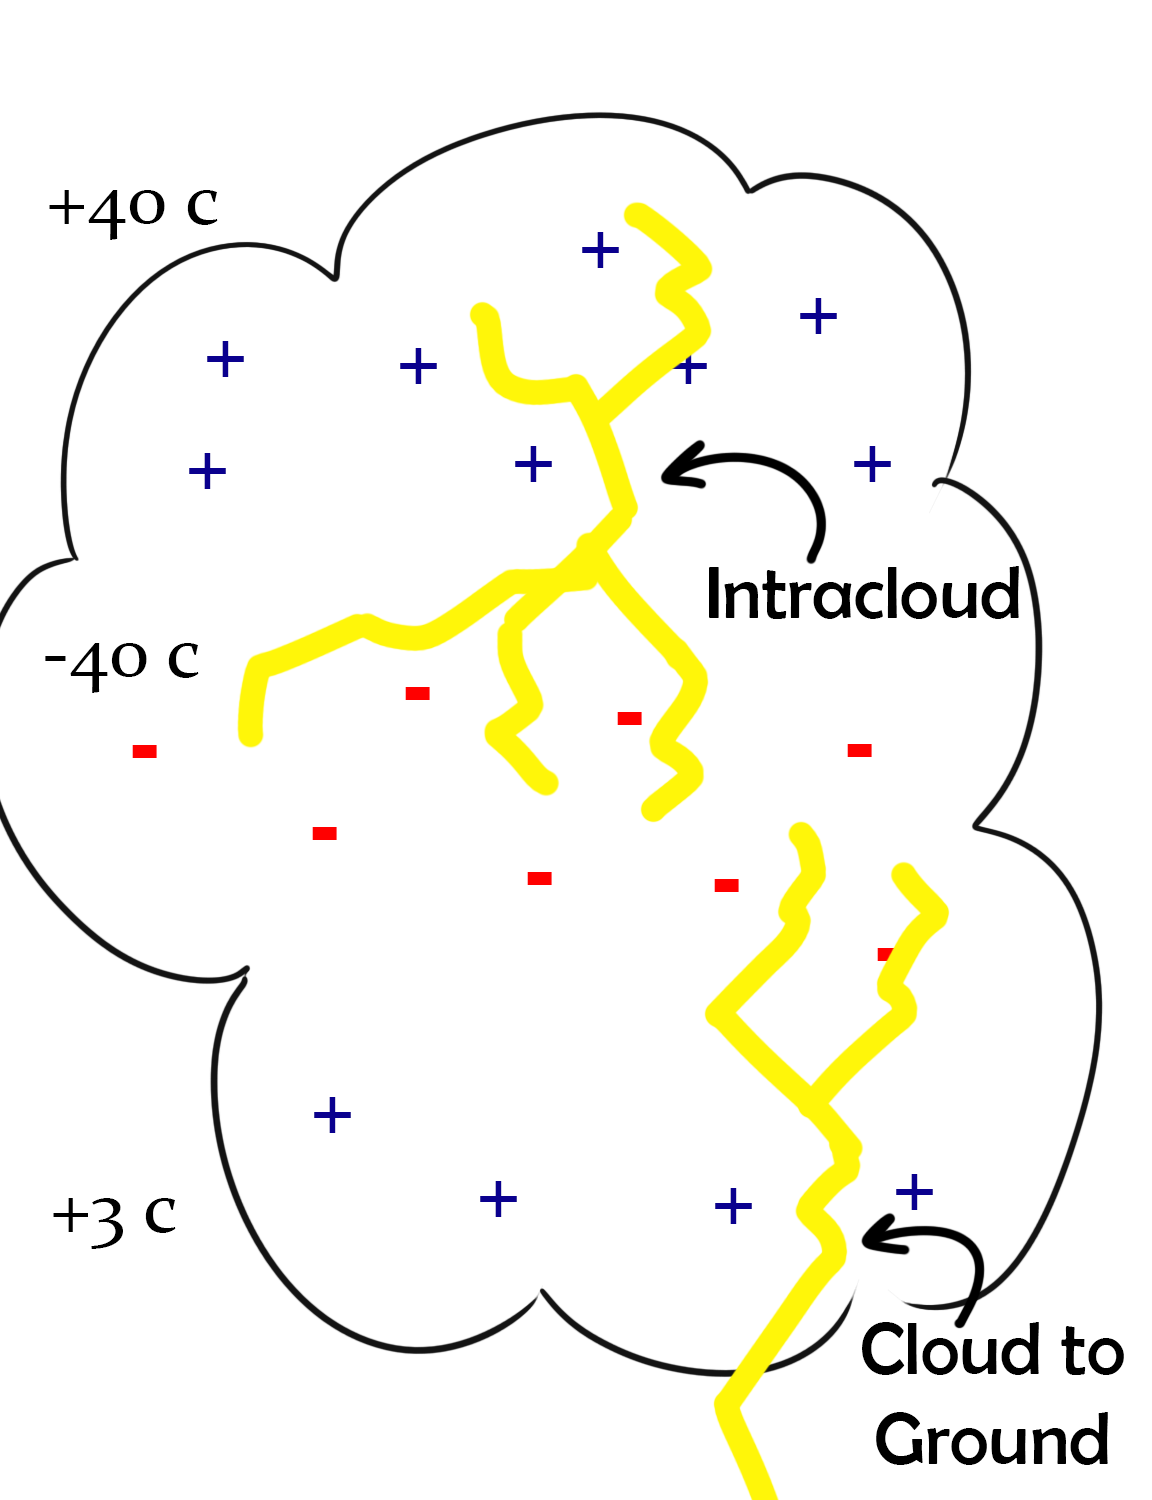
\includegraphics[width=.9\linewidth]{clouds.png}
    \end{center}
    \textbf{fig 1:} \textit{A typical charge layout of a cloud with the two most common discharge types storm clouds exhibit.}


    Lightning strikes themselves are the result of an electric breakdown in the atmospheric air between the starting and ending point. Clouds produce branches of ionized air between the cloud and the targeted surface, the most important of these branches are called step leaders. Once there is a completed path a complete circuit is created and a complete breakdown of the air happens between the two points and free electrons tear towards the lower potential.$^{5}$ The deeper interaction goes quite a bit past this, however, a basic understanding will serve us well enough to understanding RREA's. In order to ionize air in this process there is a $E_{th}$ = 2 MV/m Electric field required.${^1}$ This means that, from the limited classical model, a large electric field must be present at the starting location of the lightning strike to account for step leaders. 
    \newline
    

    \noindent
{\bf \LARGE Physics of RRE}
    
    Here is where we restate the dilemma that brought us to needing a relativistic theory to explain lighting propagation in the first place: how do we rationalize both the requirement of step leaders to initiate strikes, consequently needing a $E_{th}$ = 2 MV/m or 1-1.4 MV/m in heavy rain, while the maximum observed electric field in storm clouds is about 200 kV/m, a 1/10 of what we expect?$^{(1)}$ The answer is with a relativistic oddity: ``runaway electrons". As defined by Dwyer: ``when the rate of energy gain from an electric field exceeds the rate of energy loss from interactions with air then the energy of an electron will increase and it will `runaway.'"${(2)}$ The premise behind the physics here is moderately simple to understand. As a non-relativistic particle moves freely through a gas, in this case we are considering an electron going through a storm cloud, the mean free path will be inversely proportional to the cube of the number of particles per unit volume. However, if this particle gains enough kinetic energy, then it is allowed to start moving in a relativistic way, gaining a de Broglie wavelength that we have to consider. This wavelength allows the particle to effectively “jump” over some collisions and thus the friction the particle has with the environment will start to go down. This is what we call relativistic runaway electrons. When these electrons collide with atoms, they can knock other electrons free through Moller Scattering. These product electrons will be traveling realistically as well.$^{(1)}$ The number of relativistic runaway electrons then grow exponentially and create what is called a relativistic runaway electron avalanche. Once this avalanche reached a significantly high speed, Bremsstrahlung, reseeding events, and other high energy interactions put a limit on how much this friction can be reduced.$^{(2)}$ That will be touched in a little more detail soon. (The slope of the effective slowing force can be seen in fig 2).
    
    \noindent
    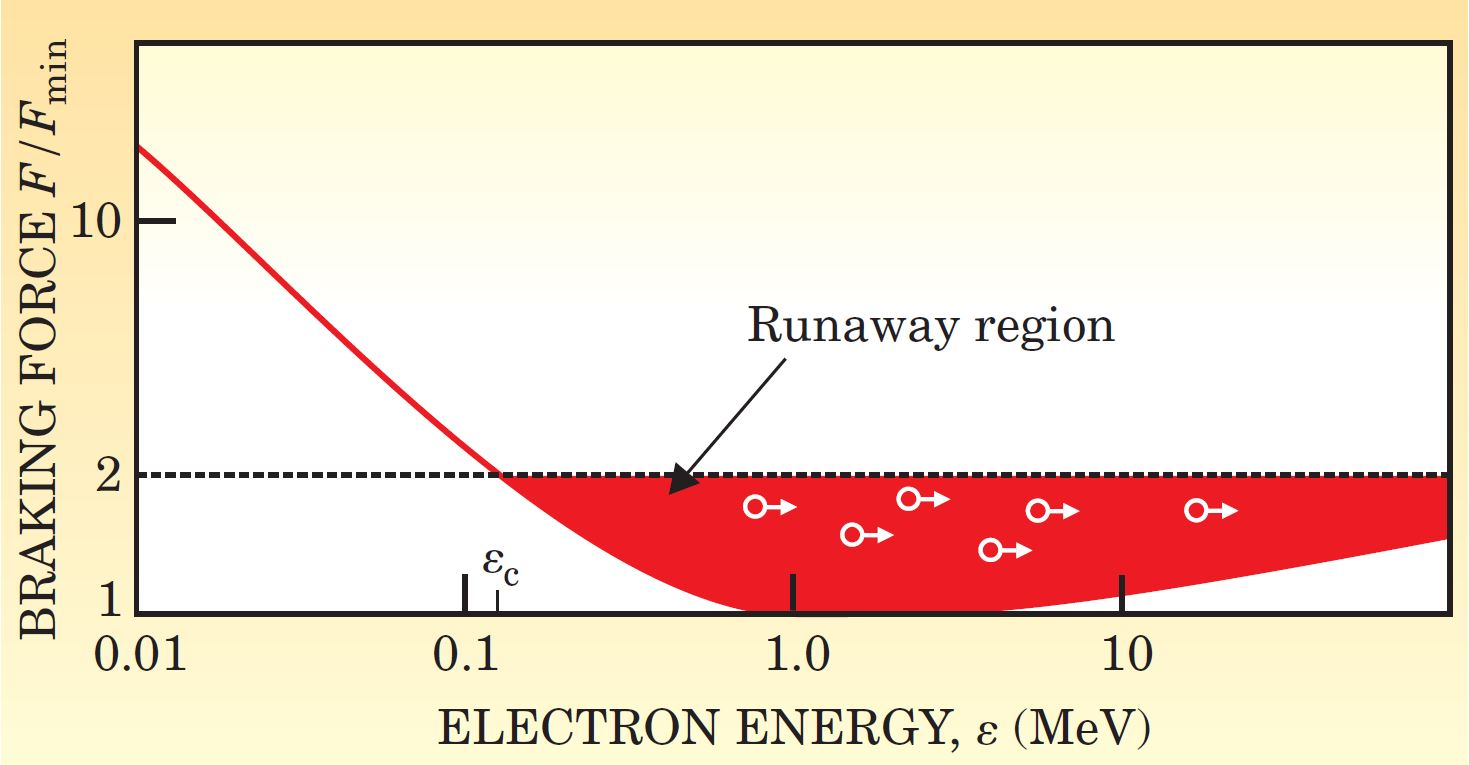
\includegraphics[width=0.5\textwidth]{images/Breaking Plot.JPG}
    \textbf{fig 2:} \textit{The evolution of breaking force with respect to the electron's energy in air. As the electron gains more kinetic energy it can decrease the effective force it feels until the breaking force is less than the accelerating force of the electric field, at this point it is in runaway. This graph was borrowed from (1).}
    
    To start these avalanches there must be a catalyst, often referred to as a seed particle. If the electric field inside the cloud is high enough then electrons can independently reach the breaking speed, this field is called the breaking field $E_b$. While the electric field within clouds are usually below this breaking field, certain hot-spots can form within the field and source seed particles for avalanches that exist outside of these initial hot-spots. These electrons are usually called `cold runaway' or `thermal runaway'.$^{(1)}$ Seed particles can also come from outside the cloud in the form of cosmic rays or radioactive decays (such as radon).$^{(3)}$ Cosmic-rays often exhibit themselves as pions traveling near the speed of light from extraterrestrial sources, like the Sun. These exotic particles quickly decay into photons, and through interactions with other atmospheric particles expand into $10^6$ to $10^{10}$ particles, in a pancake type shape.$^{(2)}$ This pancake shape is the result of the decayed photons of the pion traveling nearly horizontally to conserve four-momentum, meaning that the sum of all subsequently created particles travel a couple meters vertically while expanding out to about 100-150 m across.$^{(1)}$ Taking a closer look at this phenomena, called a Cosmic Ray Extensive Atmospheric Shower (EAS), the products in the first generation of events are about 89\% are protons, 10\% electrons, and 1\% other particles. More particles are created in subsequent generations, however they don’t play a meaningful role in the number of seed particles. So, the analysis of seed particles from cosmic rays can be considered by one generation of the EAS; and, if we consider the large number of particles involved, we can state that our observed events will have to be the product of expectable actions and not fluke probabilities.$^{(4)}$ All the interactions considered in the computational and theoretical analysis of RREA only include electrons, so the number of actual seed candidates are a magnitude lower than the total created, $10^5$-$10^9$. I should throw in a note here that ground observations have seen an increased flux of neutrons on the ground and in the air during lightning events beyond what would be expected from EAS, however these fluxes are not considered in the general RREA conversation, so I won't touch on them anymore.$^{(2)}$
    
    When an EAS is considered in the presence of a storm cloud, the number of particles created and the energy of said particles are considered as a Runaway Breakdown Extensive Atmospheric Shower (RB-EAS). A comprehensive derivation of the theoretical framework or RB-EAS was first developed by Gurevich in 2004, but the key takeaway of the phenomena was that the number of relativistic seed particles grew very quickly when the electric field of the cloud was slightly larger than the observed electric field threshold of lightning initiation (see figure 3 on the next page). Further, if energy that the electric field gives to all these seed particles is calculated, we see that the energy quickly gets out of hand. Adopting Gurevich’s terminology: $\epsilon_p$ being the cosmic ray particle energy and $\delta$ the maximum energy to threshold energy ratio $\left(\frac{E_m}{E_c}\right)$, when $\delta$ = 1.05-1.20 the energy that the particles gain from the electric field is 6-100 times that of $\epsilon_p$, and when $\delta$ = 1.4-1.6 the gained energy is $10^3$-$10^5$ times $\epsilon_p$ (see table 1 on the next page).$^{(6)}$
    
        
    Through Monte Carlo calculations, the threshold field for the a RREA was $~E_c$ = 2.83 V/m $\times n$.$^{(2)}$ We see that his value is about $130\%$ that of the breaking field. The $E_b$ value was determined as if our electron was traveling directly on the electric field lines. For most particles, however, this not the case, and through careful consideration of the angles in the theory the field inflates by a factor of $0.3$.$^{(6)}$ When compared against observational data, this $E_c$ to $E_b$ describes the upper and lower limits of the electric fields right before lightning strikes.$^{(1)}$
    
    \setstretch{1}
    \begin{center}
         \begin{tabular}{>{\centering\arraybackslash}p{0.05\textwidth}  >{\centering\arraybackslash}p{0.2\textwidth}}
         \hline
         $\delta$ & Energy W\\
         \hline
        1.05 & 61.5\\
        1.1  & 122.5\\
        1.2  & 576.6\\
        1.3  & 4510\\
        1.4  & 16844\\
        1.5  & 2.83 $\times 10^5$\\
        1.6  & 2.5  $\times 10^6$\\
        1.7  & 1.25 $\times 10^7$\\
        1.8  & 4.54 $\times 10^7$\\
        1.9  & 1.32 $\times 10^8$\\
        2.0  & 3.32 $\times 10^8$\\
         \hline
        \end{tabular}
    \end{center}
    \setstretch{2.2}
    \textbf{table 1:} \textit{The energy W given to all cosmic ray secondaries scaled to $W_0$, energy given to secondaries not in an external electric field. $W_0$ is about 0.1 of $\epsilon_p$, the initial cosmic ray energy. These values were calculated and presented by (6).}
    

    
    \begin{center}
        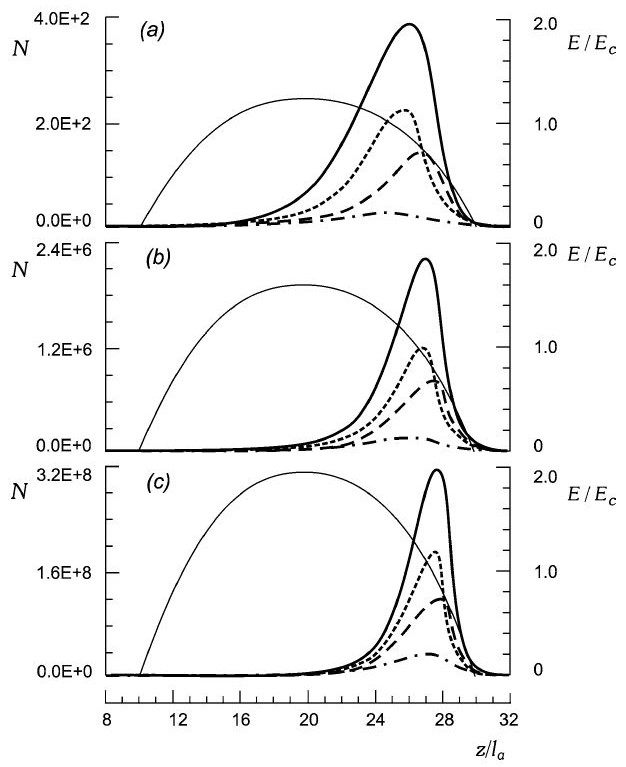
\includegraphics[width=0.95 \linewidth]{images/Dependence on relativistic electrons plot.JPG}
    \end{center}
    \textbf{fig 3:} \textit{The number of present relativistic EAS secondaries present as a function of a scaled height factor, $z/l_a$, more details about this scale can be found in the source. The $\delta$ parameter is (a) $\delta = 1.2$, (b) $\delta = 1.6$, (c) $\delta = 2.0$. The thin line shows the electric field, dashed line relativistic electrons in energy interval $1< \gamma <3$, point line $3< \gamma < 10$, dashed-point line $10< \gamma <100$, solid line is the total number of relativistic electrons. This graph was borrowed from (6).}
    
    At this point I will interject an important clarifying point made by Dwyer: while a lot of texts use the term ``runaway breakdown", the term can serve as a misnomer in this setting.$^{(2)}$ In the context of electromagnetism, breakdown often refers to the breakdown of a loop that is self-sustaining in some way.$^{(5)}$ While a RREA has a feedback system that allows for it to last for a prolonged time, it is still reliant on the background magnetic field to create this feedback loop. So, calling these events ``breakdowns" is potentially misleading. While the distinction is an important one to recognize, I trust my audience will be able discern the difference and I will use the term runaway breakdown to stay consistent with the terminology some author's use.
    
    Once a RREA is in action they will propagate until they reach some type of steady state. This steady state for one avalanche is defined as the avalanche rate. This avalanche length is the result of an unstable feedback loop. While the RRE travel though the air they can undergo EM interactions, namely compton scattering, the photoelectric effect, pair production and rayleigh scattering. When the electrons have 100keV to several MeV the primary reaction is Compton scattering, which, after accounting for subsequent interaction right after the initial production, provides photons with an energy ~100keV. When the energy of the electron is below 100keV the primary interaction is the photoelectric effect, where the photon is consumed and doesn't go on to cause any other interactions. And the final option is if the energy is above several MeV. In this case the electron undergoes pair production, creating an electron and a positron. Notice that rayleigh scattering is not in that list, and that is because it only redirect photons, and thus has little effect on the state of the avalanche. In the first case, when compton back-scattering happens, the photon can be ejected so that it reenters the avalanche area and is able to excite another electron that will be able to act as the seed particle to another avalanche. In pair production, the positron starts swimming the opposite direction of the RREA until it get outside of the avalanche area, where it is able to interact with thermal electrons and start another avalanche through Bhabha scattering with an electron.$^{(2)}$ When considering these feedback loop, it is easy to see that the number of avalanches, when existing in a moderately sized electric field, will grow exponentially. These positive feedback loops are very unstable, and thus don't continue on forever eventually capping at an average particle energy of ~7MeV.${(1)}$ The large flux of escaping photons from compton scattering and bremsstrahlung in these chain reactions have been proposed as the source of Terrestrial Gamma ray Flashes (TGFs), but more on that later. 
    \newline
    

    \noindent
{\bf \LARGE Emissions and Step Leaders}
    
    One of the first applicable uses of RREA theory is how Cosmic Ray EAS initiate short lived RREA to create Narrow Bipolar Events (NBEs). When the electric field inside a storm cloud cannot properly fuel the exponential growth of the number of avalanches, RREAs created from Cosmic Ray EAS seeds are short lived with a lifetime on the order of $\mu s$.$^{(2)}$ These quick fluxes of electron flow give pulses of current that grow exponentially with the avalanche effect, but the unstable avalanche then decays at an exponential rate. This gives a very strong radio bipolar spike that last only a couple $\mu s$.$^{(1)}$ These strong spikes are in same range as many power grid components and atmospheric devices observational devices, making interference a common occurrence. The solution to this issue is often to wrap the electrical components in a faraday cage, but is known to be a common hurdle in fine data gathering. 
    
    It has been proposed that when the avalanches exist in an environment supporting exponential growth, they source terrestrial gamma ray events. There are two flavors of these events: long emission times of around a second range, called Gamma-ray glows, and short emission times around the $\mu s$ range, called terrestrial gamma ray flashed (TGFs). As feedback events happen in the propagation of RREAs, a fraction of these photons will be leaked out of the storm cloud and describe a glowing event around clouds.${(1)}$ A standing issue with this theory is that the observed photon wavelengths from glows are considerably lower than what would be created by RREA. So while the existence of storm cloud glows are well described by the RREA mechanism, there is no definitive understanding on why we see the spectrum that we do.$^{(1)}$ The microseconds leading up to a lightning strike a quick spike in the x-ray spectrum is usually observed, these are TGFs (terrestrial gamma ray flashes). To properly explain how the theory explains these flashes we much take a detour to talking about RREAs and the step leader model.
    
    \begin{center}
        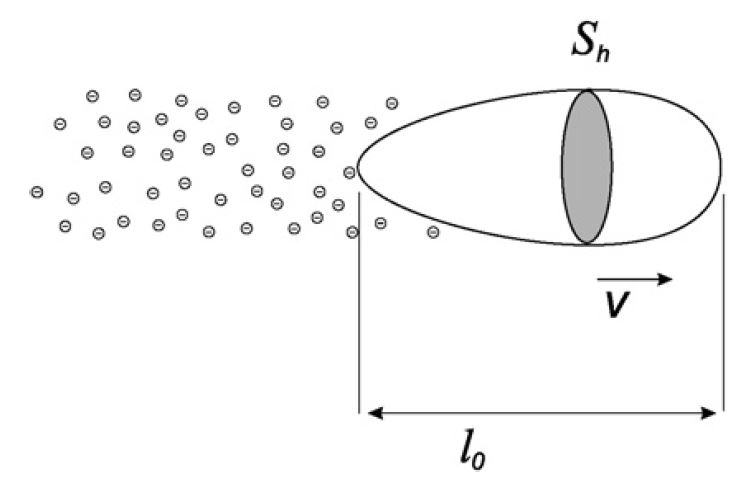
\includegraphics[width=\linewidth]{images/step leader.JPG}
    \end{center}
    \textbf{fig 4:} \textit{A depiction of Gurevich's SRB step leader model. The tear drop gets its shape from a collection of conventional breakdown effects and runaway effects. The calculated dimensions of the head are $S_h = 1-10 cm^2$, $l_0 ~ 10 cm$, $\Vec{v} \approx 6 \times 10^7 cm/s$. It should be noted that the values presented here do not agree well with laboratory observations that place $S_h ~ 10^{-2}$, this is because lab created step leaders are the product of a more forced/higher energetic process and are not detected well. All these number and graphic were borrowed from (7).}
    
    RREAs are thought to one of the main initiators in the process of lightning strikes by providing step leaders. Gurevich proposed a theoretical framework of how runaway breakdown can exist in a strong electric field.$^{(7)}$  He proposes that this field can form a teardrop like structure (see figure 4) to guild leader lines, when there is only one RREA that appears these quick flux events describe NBEs. The specifics about the dimensions of these teardrops can be see in that paper, but the important takeaways is the energy of particles and the leader's speed. In the strong electric field region created with step leaders the particle energies are 2 to 4 times the magnitude of the regular energy of runaway electrons. This large flux of electrons, and the strong magnetic field that travels with them, is about 70-100 times the breakdown field of air and is thought to be able to initiate a breakdown of air in a lightning strikes.${^{(7)}}$ The step leader's speed is limited by the speed of the avalanche speed, so the step leaders will travel in phase with the surrounding RREA events, this becomes even more important if we think about the feedback effects that will be discussed later. Dwyer does point out an issue with this theory: that the avalanche time scale described in this theory, which is proportional to $\delta^{-2/3}$,conflicts with the currently accepted observed relationship to $\delta^{-1}$. This fact does skew a couple key numbers, and the whole process is still not fully understood, but the working model assumes that feedback events puts an upper limit on this avalanche lifetime and still accepts the hypothetical frame work that Gurevich proposed.$^{(2)}$
    
    It is seen that step leaders drastically slow down in the first 15-20ns after their creation.$^{(2)}$ TGFs are a probably explanation of this phenomena. As the energetic blob of electrons moves, it quickly radiates a pulse of x-ray photons that are seen before lightning strikes.$^{(4)}$ It is important to note that TGFs are only a intra-cloud (strikes inside a thundercloud) event, as it has been conclusively shown that TGFs propagate upwards from the middle negative charge to the positive top charge of a cloud. Because of the high altitude these TGF events occur at, they were not explainable by EMP or slowly varying electric fields, which are not considerable mechanisms in large thunderclouds.$^{(2)}$ All these physical theories are quite convincing, however it should be remembered that the exact physical processes occurring during the initial upward leader propagation in an IC light flash is far from understood. Furthermore, the idea of RREA has been applied to explain other flashing events that happen lower in the cloud and in other strike types, i.e. cloud to ground, but have not provided a convincing theoretical framework yet.
    \newline


    \noindent
{\bf \LARGE Observational Data}

    \quad \quad The first production method to test RRE was done by Lehtinen in 1999, leaning almost exclusively on Moller scattering.$^{(1)}$ While the process showed good proof on concept, the model neglected to involve bremsstrahlung interactions along with many other electron interactions that would show to be crucial to explaining the processes. Within the next five years two Monte Carlo codes were written, the REAM (Runaway Electron Avalanche Model) and ELIZA by separate atmospheric physics groups. These programs introduced many interactions that were thought to be influential to the production of runaway electrons and RREAs. The current model of the codes include a laundry list of interactions:
    \begin{itemize}
        \item Runaway electrons
        \item Moller scattering
        \item Elastic scattering with coulomb shielding
        \item Bremsstrahlung production of x-rays and $\gamma$-rays and their subsequent interactions:
        \begin{itemize}
            \item Photoelectric effect
            \item Compton scattering
            \item Pair production
            \item Rayleigh scattering
        \end{itemize}
        \item Bhabha scattering
        \item All the above interaction with their positron counterparts$^{(1)}$
    \end{itemize}
    What I provided just now is not a fully comprehensive list, but provides the most notable interactions that are recognizable at the introductory level to the issue. 
    
    A common error in running these simulations and developing theory is to not apply proper limits in accordance to the physical setup. Dwyer puts it colorfully when he says many theorist have "cranked up the high-voltage knob" and applied the theory of RREAs where it doesn't belong.$^{(1)}$ As we covered earlier, different processes become dominant with different physical conditions. For example, when talking about interactions with air compton scattering dominates in the mid regime while pair production dominates in the higher energy regime. But, when all these conditions are considered carefully, the produced avalanche length, avalanche lifetime, electric field threshold, RRE speeds, and diffusion coefficients all agree well with the observed data.$^{(2)}$
    
    One of the reasons our understanding of high-energy atmospheric particle physics is so limited at this point is because of the lack of good observational data. Until modern computing, theorists relied on observed data to give a basis of new ideas and questions. With Monte Carlo and other simulation techniques that problem has been partially mitigated, but it doesn't solve the issue that we are trying to use extremely sensitive instruments to measure finite phenomena in an incredibly messy electro-magnetic environment. Through the tiresome analysis of scientist in the past, what we have been able to deduce from observational data is that RREA can only be part of the bigger picture here. Through the ionization effect of RREA, the theory can only account for about 1/10 of the total current needed to initiate a lightning strike. A proposed possible correction to this value is to consider high and low energy electrons as one population, instead of separate events.$^{(2)}$ The current theory models different tiers of electron energies (thermal electrons, those blow 100keV, those below several MeV, and those above several MeV) as mostly separate events running in parallel. The theories also divide weak and strong magnetic fields as two different stages of the process instead of allowing the two fields to interact. Once these processes are all mixed together in one algorithm, the computation time grows to an unreasonable duration. 
    
    Another barrier of work, and a primary reason our understanding of the exact processes is so limited, is that RREAs cannot be studied in the lab setting. When Wilson first brought up the idea of runaway electrons, specifically with regards to atmospheric physics, he had developed the cloud chamber for observation of this phenomena. The length scale of avalanche multiplication is on the order of hundreds of meters, which is not a feasible lab setting for a setup like a cloud chamber.$^{(5)}$ While smaller discoveries, like gamma ray flashes in smaller RRE events, have been investigated with some success, running trials on systems as large as storm clouds is outside the real for anything but a digital medium. 
    \newline
    

    \noindent
{\bf \LARGE Conclusion}
    
    Surveying the theory and computational analysis of runaway breakdown with respect to relativistic runaway electron avalanches provides some hope in the subject of high-energy atmospheric particle physics. We saw that RREs are able to cascade into avalanche effects. There are multiple possible sources of seed particles for these RREAs, from CR-EASs and electric field hot-spots; also radioactive decays of particles in the air, a topic we did not discuss. There are convincing, but incomplete, theories on how these RREAs source NBEs and intra-clouds TGFs as well as step leaders. Observational physics tells us that RREAs, as we understand them now, fit very well with some phenomena (TGFs and NBEs), but only describe a fraction of the story in other cases (such as in current initiation of lightning strikes). The simple steps described by the RREAs process can be easily summed up as the following:
    \begin{enumerate}
        \item Inhomogeneous characteristics of thunderclouds allow random cells of E-field above the break-even field of RREs to move around the cloud
        \item Seed particles enter the thundercloud, either by CR-EASs or by random excitation of a particle in the moving field
        \item These seeds allow for RREAs to begin, and are feed by positive feedback loops
        \item Some stochastic mechanics, partially described by our step leader model, allows for a discharge to occur
        \item repeat 1-4 with a random chance
    \end{enumerate}
    

% General take away from the theory? IC NBEs (strongest radio event on earth) and TFGs are well explained by it... that's about it other than good theory

% Applications of this: understating how lightning works, further understanding of RREA for fusion reactors, understand radiation emission events to protect air/space craft (dosage idea),

\end{multicols*}


    \newpage
    \noindent
{\bf \LARGE References}\\
\setlength{\parskip}{0em}


    \begin{hangparas}{.25in}{1}
    1. A.V. Gurevich, K.P. Zybin, Physics Today 58, 5, 37 (2005); doi:10.1063/1.1995746\\
    
    2. J.R. Dwyer, D.M. Smith, S.A. Cummer, Space Sci Rev (2012) 173:133–196; doi:10.1007/s11214-012-9894-0\\
    
    3. B.E. Carlson, N.G. Lehtinen, U.S. Inan, J. Geophys. Res 113 (2008) 10307; doi:10.1029/ 2008JA013210\\
    
    4. A. Chilingarian, S. Chilingaryan, \emph{et. al.}, Sci Rep. 2017 May 2;7(1):1371. doi: 10.1038/s41598-017-01288-0\\
    
    5. J.R. Dwyer, M.A. Uman, Phy Rep. 534, 4, 147-241 (2014); doi: 10.1016/j.physrep.2013.09.004\\
    
    6. A.V. Gurevich, Yu.V. Medvedev, K.P. Zybin, Phys. Lett, A 329, (2004) 348-361;\\ doi:10.1016/j.physleta.2004.06.099\\
    
    7. A.V. Gurevich, K.P. Zybin, Yu.V. Medvedev, Phys. Lett, A 361, (2007) 119-125;\\ doi:10.1016/j.physleta.2006.05.063\\
    
    8. N.S. Khaerdinov, A.S. Lidvansky, V.B. Petkov, Atmo. Res 76 (2005) 346-354;\\ doi:10.1016/j.atmosres.2004.11.012\\
    \end{hangparas}

\end{document}
